\section{Kompaktní množiny a konvergence}\label{sec:konvergence-hmp}

\begin{theorem}\label{thm:konvergence-hmp}
    Nechť $A_1,A_2,\ldots$ je nerostoucí posloupnost množin, kde $A_i\in\hyperspace(X)$ pro každé $i\in\N$. Pak posloupnost $A_1,A_2,\ldots$ konverguje k množině
    \[A=\bigcap_{i=1}^\infty A_i\]
    v Hausdorffově metrice.
\end{theorem}
\begin{proof}
    Nechť je dáno $\varepsilon>0$. Zjevně pro každé $i$ je $A\subseteq A_i$, tzn. $A\subseteq(A_i)_\varepsilon$.
    
    Nyní ukážeme, že $\hausdorffmetric(A,A_i)<\varepsilon$ pro každé $i\geqslant i_0$. Systém
    \[\mathcal{F}=\set{(A_i)_\varepsilon}\cup\set{X\setminus A_i\mid i\in\N}\]
    tvoří otevřené pokrytí množiny $A_1$ pro každé $i\in\N$. Podle předpokladu je však $A_1$ kompaktní, tedy z $\mathcal{F}$ lze vybrat konečné podpokrytí. Specificky existuje $i_0\in\N$, takové, že pro všechna $i\geqslant i_0$ je systém
    \[\mathcal{G}=\set{X\setminus A_i}\cup\set{(A)_\varepsilon}\]
    pokrytím $A_1$ a $\mathcal{G}\subseteq\mathcal{F}$ (viz obrázek \ref{fig:konvergence-hmp}). Z toho plyne, že $A_i\subseteq (A)_\varepsilon$ a tedy $\hausdorffmetric(A,A_i)<\varepsilon$.
\end{proof}
\begin{figure}[h]
    \centering
    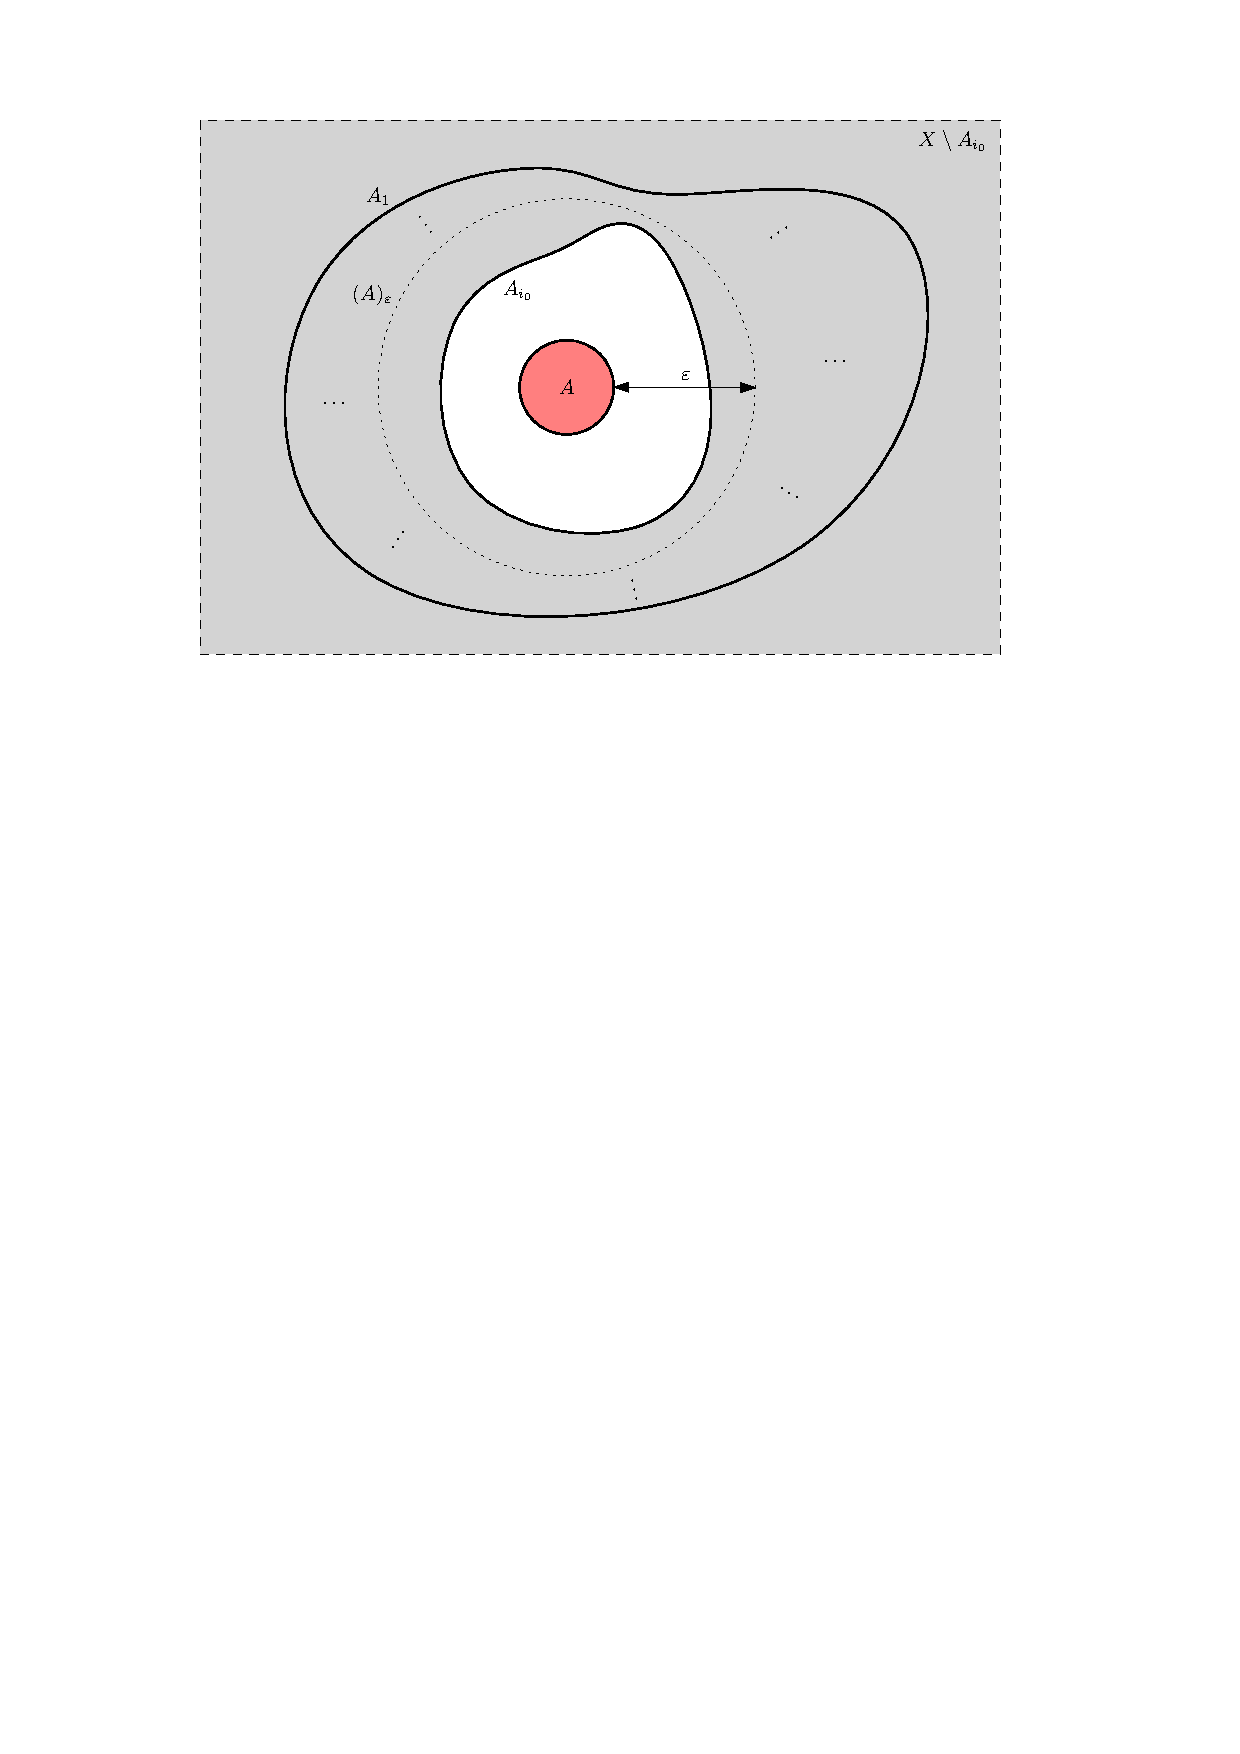
\includegraphics{ch03-ilustrace-vety-o-konvergenci.pdf}
    \caption{Ilustrace věty \ref{thm:konvergence-hmp}}
    \label{fig:konvergence-hmp}
\end{figure}

V souvislosti s konvergencí v prostoru $(\hyperspace(X),\hausdorffmetric)$ nebude na škodu si připomenout jedno známé související tvrzení z matematické analýzy.
\begin{theorem}[Cantorova]\label{thm:cantor}
    Následující tvrzení jsou ekvivalentní:
    \begin{enumerate}[label=(\roman*)]
        \item\label{thm:cantor-uplnost} $(X,\varrho)$ je úplný metrický prostor.
        \item\label{thm:cantor-nekl-posl-mnozin} Je-li $A_1,A_2,\ldots$ neklesající posloupnost uzavřených množin, kde $A_i\subseteq X$ pro každé $i\in\N$, takových, že $\diam{A_i}\to 0$, pak existuje $x\in X$ splňující
        \[\bigcap_{i=1}^\infty A_i=\set{x}.\]
    \end{enumerate}
\end{theorem}
Věta \ref{thm:cantor} je v podstatě rozšířením Cantorova principu vnořených intervalů v $\R$. Speciálně z toho vyplývá, že i v Hausdorffově metrickém prostoru platí podmínka \ref{thm:cantor-nekl-posl-mnozin}, neboť z věty \ref{thm:uplnost-hmp} víme, že $(\hyperspace(X),\hausdorffmetric)$ tvoří úplný metrický prostor.